\documentclass{article}
\usepackage[utf8]{inputenc}
\usepackage{amsmath, amsfonts, amsthm, amssymb, graphicx, geometry, lipsum}
\usepackage{hyperref}
\usepackage{indentfirst}
\usepackage[all,cmtip]{xy}
\usepackage{float}
\usepackage[numbers,square]{natbib}


\newtheorem{definition}{Definition}[section]
\newtheorem{lemma}{Lemma}[section]
\newtheorem{theorem}{Theorem}[section]
\newenvironment{theorem*}
 {\expandafter\def\expandafter\thetheorem\expandafter{\thetheorem*}\theorem}
 {\endtheorem}
\newtheorem{corollary}{Corollary}[theorem]
\newtheorem{proposition}{Proposition}[theorem]
\theoremstyle{remark}
\newtheorem*{remark}{Remark}


\newcommand{\N}{\mathbb{N}}
\newcommand{\Z}{\mathbb{Z}}
\newcommand{\Q}{\mathbb{Q}}
\newcommand{\R}{\mathbb{R}}
\newcommand{\C}{\mathbb{C}}
\newcommand{\F}{\mathbb{F}}
\newcommand{\PP}{\mathbb{P}}
\newcommand{\HH}{\mathbb{H}}
\newcommand{\norm}[1]{\left\lVert #1 \right\rVert}
\newcommand{\innerp}[2]{\langle #1, #2 \rangle}

\DeclareMathOperator{\di}{d\!}

\title{Dynamical Systems of Particles Around a Kerr Black Hole\\
{\Large University of Toronto}}
\author{Haocheng Sun}
\date{Winter 2025}


\begin{document}
\maketitle



\section{Introduction}

Black holes, as predicted by general relativity, are among the most intriguing objects in our universe. In this report, we extend the non-rotating black holes to rotating black holes described by the Kerr metric.  In 1963, Roy Kerr discovered an exact solution to Einstein's 
field equations describing a rotating, uncharged black hole. This solution has been extensively investigated due to its relevance in modeling 
astrophysical black holes, which are generally expected to have significant spin. A foundational 
overview of general relativity and its mathematical structure is provided in texts such 
as \emph{A First Course in General Relativity}~\cite{schutz} and Wald's \emph{General 
Relativity}~\cite{wald}.

This report investigates the dynamics of particles orbiting a Kerr black hole. By employing Hamiltonian and Hamilton–Jacobi formalisms, we derive key conserved quantities and analyze the motion of test particles in curved spacetime. Numerical simulations further illustrate complex phenomena, offering insights into high-energy astrophysical processes.



\section{Overview of Kerr Black Hole}

The spacetime geometry around a rotating black hole is described by the Kerr metric. In this study, we adopt the Boyer-Lindquist coordinates \((t, r, \theta, \phi)\), which conveniently represent the stationary and axisymmetric properties of Kerr spacetime. The metric components and detailed descriptions can be found in \emph{A First Course in General Relativity}~\cite{schutz}. For simplicity, we will set $G=c=1$.
\begin{align}\label{eq:kerr-metric}
    ds^2 = \;& -\frac{\Delta - a^2 \sin^2\theta}{\Sigma} \, dt^2
    - 2 a \sin^2\theta \,\frac{r^2 + a^2 - \Delta}{\Sigma} \, dt \, d\phi \nonumber \\
    & + \frac{\Sigma}{\Delta} \, dr^2+ \Sigma \, d\theta^2
    + \frac{(r^2 + a^2)^2 - \Delta \, a^2 \sin^2\theta}{\Sigma} \, \sin^2\theta \, d\phi^2
\end{align}
where $\Sigma$ and $\Delta$ are defined as
\begin{align}
    \Sigma &= r^2 + a^2 \cos^2\theta\\
    \Delta &= r^2 + a^2 - 2 M r
\end{align}
The black hole's spin (or rotation) parameter is defined as $a = \frac{J}{M}$
where $J$ is the total angular momentum of the black hole, and $M$ is the black hole mass in geometrized units ($c = G = 1$). In these units, $a$ has the dimension of length. If $a = 0$, the black hole is nonrotating (a Schwarzschild black hole). When $a \neq 0$, the black hole is rotating.



We already know that a non-rotating black hole has a single event horizon, leading to a simple overall structure. But for a Kerr black hole, there is a unique region called the ergosphere, within which spacetime is dragged by the black hole’s rotation so that no object can remain stationary relative to a distant observer.  

\begin{equation}
    r_{\text{ergosphere}}=M + \sqrt{M^2-a^2\cos^2{\theta}}
\end{equation}

Furthermore, the Kerr black hole possesses two horizons (an outer event horizon and an inner Cauchy horizon) 

\begin{equation}
    r_+ = M + \sqrt{M^2 - a^2}    
\end{equation}
\begin{equation}
    r_- = M - \sqrt{M^2 - a^2}
\end{equation}
and a ring-shaped singularity, making its internal configuration more intricate than that of a non-rotating black hole, which has only one horizon and a point-like singularity. 
\begin{figure}[htbp] 
    \centering          
    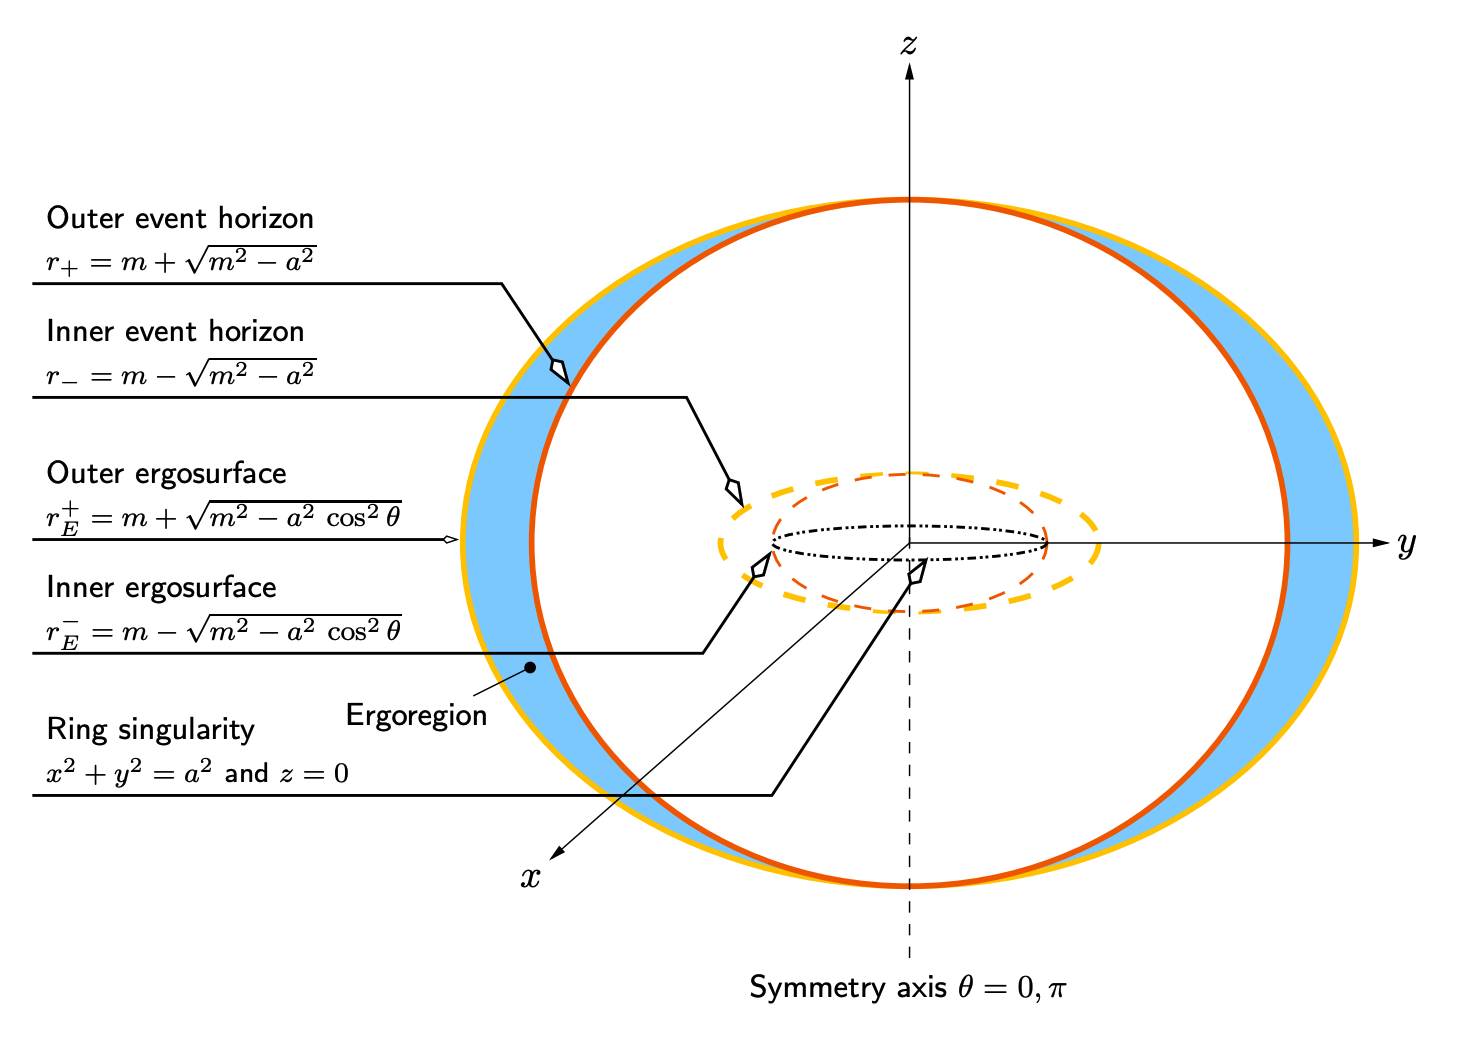
\includegraphics[width=0.8\textwidth]{Kerr Black Hole.png}
    \caption{Schematic Kerr Black Hole~\cite{visser}}
    \label{KBH}
\end{figure}

In terms of symmetry, the Kerr solution is only axisymmetric because of its spin, whereas the non-rotating (Schwarzschild) solution is fully spherically symmetric. Overall, the rotation of the Kerr black hole introduces additional complexities such as frame dragging and the ergosphere, while the non-rotating black hole remains simpler and more symmetric. Notably, when the Kerr black hole’s spin parameter approaches zero, its description reduces to the Schwarzschild solution.

\section{Mathematical Description of the Dynamical System}


We assumed the Kerr black hole to be stationary, so the metric is independent of the time, and we have a Killing vector $k=(1,0,0,0)$. Also, we assume the black hole to be axisymmetric; without loss of generality, we assume it rotates around the z-axis. So we have another Killing vector $m=(0,0,0,1)$.
As always, for a geodesic with affine parameter $\lambda$, we use $x$ to denote the position of the geodesic, just keep in mind that we are working with Boyer-Lindquist coordinates. We use $u$ to denote the velocity vector.

\begin{definition}
    We first define the \textit{Lagrangian} to be 
    \begin{equation}
        \mathcal{L}\bigl(x, \dot{x}\bigr) \;:=\; \frac{1}{2}g(\dot{x},\dot{x})
=\frac{1}{2}g_{\mu\nu}\dot{x}^\mu\,\dot{x}^\nu
    \end{equation}
Also, we define the \textit{conjugate momentum} $p_\mu$ as
\begin{equation}
p_\mu \;:=\; \frac{\partial \mathcal{L}}{\partial \dot{x}^\mu}
\;=\; g_{\mu\nu}\,\dot{x}^\nu,
\end{equation}
\end{definition}

Notice that the physical momentum $p^{\mu}=u^{\mu}$, so lowering the index we have $p_{\mu}=g_{\mu\nu}u^{\nu}$ which is just the conjugate momentum defined above.

\begin{lemma}
    $p_t$ and $p_{\phi}$ are constant along the geodesics.
\end{lemma}
\begin{proof}
    Let $\xi$ denote any of the two Killing vectors above. By the Killing vector equation 
    \begin{equation}
        \nabla_{\mu}\xi_{\nu}+\nabla_{\nu}\xi_{\mu}=0
    \end{equation}
    Since $u=p$, and by the geodesic equation
    \begin{equation}
        p^{\nu}\nabla_{\nu}p_{\mu}=u^{\nu}\nabla_{\nu}u_{\mu}=0
    \end{equation}
    So consider how $\xi_{\mu}p^{\mu}$ changes along the geodesic, we have
    \begin{align}
        p^{\nu}\nabla_{\nu}(\xi_{\mu}p^{\mu}) &= p^{\nu}[(\nabla_{\nu}\xi_{\mu})p^{\mu} + \xi_{\mu}(\nabla_{\nu}p^{\mu})]\\
        &= p^{\nu}(\nabla_{\nu}\xi_{\mu})p^{\mu}\\
        &= \frac{1}{2}p^{\nu}p^{\mu}(\nabla_{\nu}\xi_{\mu}) + \frac{1}{2}p^{\nu}p^{\mu}(-\nabla_{\mu}\xi_{\nu})\\
        &=0
    \end{align}
\end{proof}
So the geodesic motion in Kerr geometry gives us two constants $p_t$ and $p_{\phi}$. The energy and angular momentum are $E=-k^{\mu}u_{\mu}$ and $L=m^{\mu}u_{\mu}$. Hence, it is easy to see that $E=-p_t$ and $L=p_{\phi}$ are constant along the geodesic. We should not forget there is another trivial invariant $\kappa$ which is the invariant mass of the test particle, defined by 
\begin{equation}
    \kappa = g_{\mu\nu}u^{\mu}u^{\nu}=g_{\mu\nu}p^{\mu}p^{\nu}
\end{equation}
\[
\kappa \;=\;
\begin{cases}
-1 & \text{for timelike geodesics},\\[6pt]
+1 & \text{for spacelike geodesics},\\[6pt]
0  & \text{for null geodesics}.
\end{cases}
\]


In this section, we are going to show that there is another constant $Q$ by using the Hamilton--Jacobi theory, and it was originally proved by Brandon Carter in his paper \emph{Global Structure of the Kerr Family of Gravitational Fields}~\cite{carter}.

\begin{definition}\label{def:carter}
    We define
    \begin{equation}
        Q :=
    p_{\theta}^2
    \;-\;
    \cos^2 \theta \,
    \biggl[
    (\kappa + E^2)\,a^2
    \;-\;
    \frac{L^2}{\sin^2 \theta}
    \biggr]
    \end{equation}

\end{definition}

\begin{definition}
    We define the Hamiltonian to be a function of the coordinate and the conjugate momentum:
    \begin{align}
        H(x^0,\cdots,x^3,p_0,\cdots,p_3) &:= p_{\mu}\dot{x}^{\mu}-\mathcal{L}(x,\dot{x})\label{eq:legendre}\\
        &= p_{\mu}g^{\mu\nu}p_{\nu} - \frac{1}{2}g_{\mu\nu}\dot{x}^{\mu}\dot{x}^{\nu}\\
        &= p_{\mu}g^{\mu\nu}p_{\nu} - \frac{1}{2}g_{\mu\nu}g^{\mu\alpha}p_{\alpha}g^{\nu\beta}p_{\beta}\\
        &= \frac{1}{2}p_{\mu}g^{\mu\nu}p_{\nu}
    \end{align}
\end{definition}
By easy computation, we have the Hamiltonian equations
\begin{align}
\dot{x}^\mu &= \frac{\partial H}{\partial p_\mu}\label{eq:hamilton-x}\\
\dot{p}_\mu &= -\,\frac{\partial H}{\partial x^\mu}\label{eq:hamilton-p}
\end{align}
But solving this system of equations is not an easy job. So as mentioned above, here we use the Hamilton--Jacobi approach.


\begin{theorem}[Jacobi]\label{thm:jacobi}
    Let $S(x,\lambda)$ be a solution of the Hamilton--Jacobi equation
    \begin{equation}
        H\!\Bigl(x, \frac{\partial S}{\partial x}\Bigr)
        + \frac{\partial S}{\partial \lambda} = 0
    \end{equation}
    where $\frac{\partial S}{\partial x}=(\frac{\partial S}{\partial x^0},\cdots,\frac{\partial S}{\partial x^3})$. Let $x(\lambda)$ be a curve satisfying $\dot{x}^{\mu} = \frac{\partial H}{\partial p_{\mu}}\bigl(x, \frac{\partial S}{\partial x}\bigr)$, and set $p_{\mu}(\lambda) := \frac{\partial S}{\partial x^{\mu}}\bigl(x(\lambda),\lambda\bigr)$. Then $\bigl(x(\lambda), p(\lambda)\bigr)$ satisfies Hamilton's equations, so $x(\lambda)$ is a geodesic, and along it
    \begin{equation}
        \frac{\partial S}{\partial x^{\mu}} = p_{\mu}
    \end{equation}
    \begin{equation}
        \frac{\partial S}{\partial \lambda} = -H
    \end{equation}
\end{theorem}
\begin{proof}
    The first Hamilton equation holds by construction. For the second, we differentiate $p_{\mu}$ along the curve:
    \begin{equation}
        \dot{p}_{\mu} = \frac{\partial^2 S}{\partial x^{\mu}\partial x^{\nu}}\,\dot{x}^{\nu} + \frac{\partial^2 S}{\partial x^{\mu}\partial \lambda}
    \end{equation}
    On the other hand, differentiating the Hamilton--Jacobi equation with respect to $x^{\mu}$ gives
    \begin{equation}
        \frac{\partial H}{\partial x^{\mu}} + \frac{\partial H}{\partial p_{\nu}}\frac{\partial^2 S}{\partial x^{\nu}\partial x^{\mu}} + \frac{\partial^2 S}{\partial \lambda\,\partial x^{\mu}} = 0
    \end{equation}
    Since $\frac{\partial H}{\partial p_{\nu}} = \dot{x}^{\nu}$, comparing the two equations yields $\dot{p}_{\mu} = -\frac{\partial H}{\partial x^{\mu}}$. Finally, $\frac{\partial S}{\partial \lambda} = -H$ is just the Hamilton--Jacobi equation evaluated along the curve.
\end{proof}

\begin{remark}
    The Hamilton--Jacobi equation is not an arbitrary choice: it is satisfied by the action itself, which is the converse direction of Theorem~\ref{thm:jacobi}. Fix an initial point $x_0$ at $\lambda_0$, and let
    \begin{equation}
        S(x,\lambda)=\int_{\lambda_0}^{\lambda} \mathcal{L}\,d\lambda'
    \end{equation}
    be the action along the solution of the Euler--Lagrange equations from $x_0$ to $x$ (Hamilton's principal function, see \emph{Classical Mechanics, Chapter 10}~\cite{goldstein}). Then $\frac{\partial S}{\partial x^{\mu}} = p_{\mu}$ and $\frac{\partial S}{\partial \lambda} = -H$; in particular, $S$ solves the Hamilton--Jacobi equation.
\end{remark}
\begin{proof}
    We vary the endpoint $x$ while keeping $x_0$ fixed. The variation in $S$ is
    \begin{equation}
        \delta S 
        = 
        \int_{\lambda_0}^{\lambda} 
        \biggl(
           \frac{\partial \mathcal{L}}{\partial x^\mu}\,\delta x^\mu
           \;+\;
           \frac{\partial \mathcal{L}}{\partial \dot{x}^\mu}\,\delta \dot{x}^\mu
        \biggr)
        \,d\lambda
    \end{equation}
    The trajectories obey the Euler-Lagrange equation and we must have
    \begin{equation}
        \frac{\partial \mathcal{L}}{\partial x^{\mu}} = \frac{d}{d\lambda}\frac{\partial \mathcal{L}}{\partial \dot{x}^{\mu}}
    \end{equation}
    on the other hand $\delta \dot{x} = \frac{d}{d\lambda}(\delta x)$. Using these relations, we can rewrite the variation of $S$ as
    \begin{align}
        \delta S &= \int_{\lambda_0}^{\lambda} \left(\frac{\partial \mathcal{L}}{\partial \dot{x}}\frac{d(\delta x)}{d\lambda} + \frac{d}{d\lambda}(\frac{\partial \mathcal{L}}{\partial \dot{x}})\delta x\right)d\lambda \\
        &= \int_{\lambda_0}^{\lambda}\frac{d}{d\lambda}\left( \frac{\partial \mathcal{L}}{\partial \dot{x}}\delta x\right)d\lambda\\
        &= \left[\frac{\partial \mathcal{L}}{\partial \dot{x}}\delta x \right]_{\lambda_0}^{\lambda}\\
        &= p_\mu(\lambda)\,\delta x^\mu(\lambda)
          \;-\;
          p_\mu(\lambda_0)\,\delta x^\mu(\lambda_0)
    \end{align}
    Since the initial endpoint is fixed, \(\delta x^\mu(\lambda_0) = 0\). Hence,
    \begin{equation}
        \delta S 
        = p_\mu(\lambda)\,\delta x^\mu(\lambda)
            \end{equation}
    Comparing the coefficients of \(\delta x^\mu(\lambda)\) on both sides, 
    we obtain
    \begin{equation}
        \frac{\partial S}{\partial x^\mu} 
        = p_\mu
    \end{equation}
    On the other hand, by the definition of $S$, we have $\frac{dS}{d\lambda} = \mathcal{L}$ along the actual trajectory \(x^\mu(\lambda)\). Computing the same total derivative of \(S\bigl(x^\mu(\lambda), \lambda\bigr)\) by the chain rule and using \eqref{eq:legendre}:
    \begin{equation}
        \frac{dS}{d\lambda}
        = \frac{\partial S}{\partial x^\mu}\,\dot{x}^\mu
          + \frac{\partial S}{\partial \lambda}
        = p_\mu \,\dot{x}^\mu
          + \frac{\partial S}{\partial \lambda}
          = H+\mathcal{L}+ \frac{\partial S}{\partial \lambda}
    \end{equation}
    Hence we also have 
    \begin{equation}
        \frac{\partial S}{\partial \lambda} = -H
    \end{equation}
\end{proof}
Therefore, by Theorem~\ref{thm:jacobi}, once we have a solution $S$, the conjugate momenta $p_{\mu}=\frac{\partial S}{\partial x^{\mu}}$ and hence $\dot{x}^{\mu}$ are determined, and the geodesic equations reduce to first-order equations.

Since $H$ does not depend explicitly on $\lambda$, $t$ or $\phi$, it is natural to look for solutions of the Hamilton--Jacobi equation in which these variables separate. This is an ansatz, not a consequence of Theorem~\ref{thm:jacobi}.

\begin{corollary}
    Suppose $S$ solves the Hamilton--Jacobi equation and has the separated form
    \begin{equation}\label{eq:ansatz}
        S 
        = 
        -\tfrac{1}{2}\,\kappa\,\lambda
        \;-\;
        E\,t
        \;+\;
        L\,\phi
        \;+\;
        S^{(r\theta)}(r,\theta)
    \end{equation}
    where $\kappa$, $E$, $L$ are constants and \(S^{(r\theta)}\) is a function of \(r\) and \(\theta\) to be determined. Then along the geodesics of Theorem~\ref{thm:jacobi}, $g^{\mu\nu}p_{\mu}p_{\nu}=\kappa$, $p_t=-E$ and $p_{\phi}=L$; that is, the separation constants are exactly the conserved quantities found above.
\end{corollary}
\begin{proof}
    By Theorem~\ref{thm:jacobi}, $\frac{\partial S}{\partial x^{\mu}} = p_{\mu}$ and $\frac{\partial S}{\partial \lambda} = -H$ along the geodesic. Differentiating \eqref{eq:ansatz} gives
    \begin{equation}
        \frac{\partial S}{\partial \lambda} = -H = -\frac{1}{2}g^{\mu\nu}p_{\mu}p_{\nu}=-\frac{1}{2}\kappa
    \end{equation}
    \begin{equation}
        \frac{\partial S}{\partial t}=p_t = -E
    \end{equation}
    \begin{equation}
        \frac{\partial S}{\partial \phi}=p_{\phi} = L
    \end{equation}
\end{proof}
\begin{theorem}
    The quantity $Q$ we defined is also constant along geodesics, it is called the Carter constant.
\end{theorem}
\begin{proof}
We follow the idea of B. Carter~\cite{carter}, we want to find a separable solution, so we further assume $S$ has the following expression
    \begin{equation}
        S \;=\; -\,\tfrac12\,\kappa\,\lambda
        \;-\; E\,t
        \;+\; L\,\phi
        \;+\; S^{(r)}(r)
        \;+\; S^{(\theta)}(\theta)
    \end{equation}
We now want to substitute this expression into the Hamilton--Jacobi equation. In order to do this, we first compute that the inverse of the Kerr metric is 
\begin{equation}
    g^{-1}
\;=\;
\begin{pmatrix}
-\frac{1}{\Delta} \bigl[r^2 + a^2+\frac{2Mra^2\sin^2\theta}{\Sigma}\bigr] & 0 & 0 & -\,\frac{2\,M\,r\,a}{\Sigma\,\Delta}\\[6pt]
0 & \displaystyle \frac{\Delta}{\Sigma} & 0 & 0\\[6pt]
0 & 0 & \displaystyle \frac{1}{\Sigma} & 0\\[6pt]
-\,\frac{2\,M\,r\,a}{\Sigma\,\Delta} & 0 & 0 & \frac{\Delta \;-\; a^2\sin^2\theta}{\Sigma\,\Delta\;\sin^2\theta}
\end{pmatrix}
\end{equation}
Also by the expression $H=\frac{1}{2}p_{\mu}g^{\mu\nu}p_{\nu}$, the H-J equation reduces to 
\begin{equation}
    \frac{1}{2}\frac{\partial S}{\partial x^{\mu}}g^{\mu\nu}\frac{\partial S}{\partial x^{\nu}}+\frac{\partial S}{\partial \lambda}=0
\end{equation}
\begin{equation}
    -\kappa
+
\frac{\Delta}{\Sigma}\Bigl(\frac{dS^{(r)}}{dr}\Bigr)^{2}
+
\frac{1}{\Sigma}\,\Bigl(\frac{dS^{(\theta)}}{d\theta}\Bigr)^{2}
-
\frac{1}{\Delta}\,\biggl[
  r^{2} + a^{2}
  +
  \frac{2Mra^{2}\sin^{2}\theta}{\Sigma}
\biggr]E^{2}
+
\frac{4Mra}{\Sigma\,\Delta}EL
+
\frac{\Delta - a^{2}\sin^{2}\theta}{\Sigma\Delta\sin^{2}\theta}L^{2}
=0
\end{equation}
Notice that
\begin{align}
(r^2 + a^2)+\frac{2\,M\,r\,a^2\,\sin^2\theta}{\Sigma}
&=\frac{1}{\Sigma}
\bigl[
  (r^2 + a^2\cos^2\theta)(r^2 + a^2)+2Mra^2\sin^2\theta
\bigr]
\\
&=
\frac{1}{\Sigma}
\bigl[
  (r^2 + a^2)^2-(r^2 + a^2)^2\sin^2\theta+
  2Mra^2\sin^2\theta
\bigr]
\\
&=
\frac{1}{\Sigma}
\bigl[
  (r^2 + a^2)^2-a^2\sin^2\theta\Delta
\bigr]
\end{align}
Substitute the equation above into the H-J equation and multiplying by $\Sigma$ we have:
\begin{equation}
    -\kappa\Sigma
+ \Delta\bigl(\tfrac{dS^{(r)}}{dr}\bigr)^2 + \bigl(\tfrac{dS^{(\theta)}}{d\theta}\bigr)^2
- \Bigl[\tfrac{(r^2 + a^2)^2}{\Delta}- a^2\sin^2\theta\Bigr]E^2
+ \tfrac{4Mra}{\Delta}EL
+ \Bigl[\tfrac{1}{\sin^2\theta} - \tfrac{a^2}{\Delta}\Bigr]L^2
= 0
\end{equation}
The equation above only involves $r$ and $\theta$, so we rearrange the equation such that the LHS only involves $r$ while the RHS only involves $\theta$
\begin{equation}
    \Delta\Bigl(\frac{dS^{(r)}}{dr}\Bigr)^2- \kappa r^2
    - \frac{(r^2 + a^2)^2}{\Delta}E^2
    + \frac{4Mra}{\Delta}EL
    - \frac{a^2L^2}{\Delta}
    =
    -\Bigl(\frac{dS^{(\theta)}}{d\theta}\Bigr)^2
    + \kappa\,a^2\cos^2\theta
    - a^2\sin^2\theta E^2
    - \frac{1}{\sin^2\theta}L^2
\end{equation}
By our definition of $Q$, we see that 
\begin{equation}
    -Q = -(\frac{\partial S}{\partial \theta})^2 + \kappa a^2 \cos^2\theta + a^2\cos^2\theta E^2 -\frac{L^2}{\sin^2\theta}\cos^2\theta
\end{equation}
which is very similar to the RHS of the equation above. In order to make the RHS$=-Q$, we add $a^2E^2+L^2$ to both sides, so the equation becomes
\begin{equation}
    \Delta\Bigl(\frac{dS^{(r)}}{dr}\Bigr)^2
    -\kappa r^2
    -\frac{(r^2 + a^2)^2}{\Delta}E^2
    +\frac{4Mra}{\Delta}EL
    -\frac{a^2 L^2}{\Delta} +a^2 E^2 +L^2 = -Q
\end{equation}
Since $Q$ is independent of $r$, and by the expression above, $Q$ is also independent of $\theta$, therefore it is also a constant.

It remains to check that this constant is conserved along an arbitrary geodesic. Given any geodesic, choose $\kappa$, $E$, $L$ and $Q$ from its initial momentum, and choose the signs of $\frac{dS^{(r)}}{dr}$ and $\frac{dS^{(\theta)}}{d\theta}$ to match those of $p_r$ and $p_{\theta}$, so that $\frac{\partial S}{\partial x^{\mu}} = p_{\mu}$ at the initial point. By Theorem~\ref{thm:jacobi} and the uniqueness of solutions of Hamilton's equations, the geodesic is the curve generated by $S$, so $p_{\theta} = \frac{dS^{(\theta)}}{d\theta}$ along it, and the quantity $Q$ of Definition~\ref{def:carter} keeps its initial value. At turning points, where $p_r$ or $p_{\theta}$ vanishes, the sign of the corresponding square root switches; since $Q$ is continuous along the geodesic, it remains constant.
\end{proof}




\begin{theorem}\label{thm:R}
We define the functions $R(r)$ and $\Theta(\theta)$ as:
    \begin{equation}
        R(r)=\Delta\Bigl[\kappa r^2-(L - aE)^2-Q\Bigr]
        +\Bigl[E(r^2 + a^2)-La\Bigr]^2
    \end{equation}
    \begin{equation}
        \Theta(\theta)=Q+\cos^2\theta
        \Bigl[(\kappa + E^2)a^2-\frac{L^2}{\sin^2\theta}\Bigr]
    \end{equation}
    Then we have the following two ODEs:
    \begin{equation}
        p_{\theta}^2 \;=\; \bigl(\Sigma\,\dot{\theta}\bigr)^2 \;=\; \Theta(\theta),
        \quad
        p_{r}^2 \;=\; \Bigl(\tfrac{\Sigma}{\Delta}\,\dot{r}\Bigr)^2 \;=\; \tfrac{R(r)}{\Delta^2}
    \end{equation}

\end{theorem}
\begin{proof}
    $p_{\theta}^2=\Theta(\theta)$ follows immediately after the expression of $Q$. Also, by the metric of Kerr spacetime
    \begin{equation}
        p_{\theta} = g_{\theta\nu}\dot{x}^{\nu}=g_{\theta\theta}\dot{\theta}=\Sigma \dot{\theta}
    \end{equation}
    Now consider $p_r$, we already know that
    \begin{equation}
    \Delta\Bigl(\frac{dS^{(r)}}{dr}\Bigr)^2
    -\kappa r^2
    -\frac{(r^2 + a^2)^2}{\Delta}E^2
    +\frac{4Mra}{\Delta}EL
    -\frac{a^2 L^2}{\Delta} +a^2 E^2 +L^2 = -Q
    \end{equation}
    Notice that 
    \begin{equation}
        \frac{4Mra}{\Delta}EL = \frac{2aLE}{\Delta}\cdot 2Mr= \frac{2aLE}{\Delta}(r^2+a^2-r^2-a^2+2Mr)= \frac{2aLE}{\Delta}(r^2+a^2-\Delta)
    \end{equation}
    Therefore, using this result and the definition of $R(r)$, we get
    \begin{equation}
        p_r^2 = \frac{R}{\Delta^2}
    \end{equation}
    Similarly, using the metric of Kerr spacetime, we immediately have $p_r=\frac{\Sigma}{\Delta}\dot{r}$
\end{proof}


\begin{theorem}\label{thm:tphi}
    For the parameters $\phi$, $t$ of the geodesics, we have the following expression:
    \begin{equation}
        \Sigma\dot{\phi} = -(a E-\frac{L}{\sin^2\theta})+\frac{a}{\Delta}[E(r^2+a^2)-aL]
    \end{equation}    
    \begin{equation}
        \Sigma \dot{t} = -(a^2 E \sin^2\theta-aL) + \frac{r^2+a^2}{\Delta}[E(r^2+a^2)-aL]
    \end{equation}
\end{theorem}
\begin{proof}
By solving the system of ODEs below:
    \begin{equation}
        \begin{cases}
            p_t = g_{tt}\dot{t} +g_{t\phi}\dot{\phi} = -E \\
            p_\phi = g_{\phi t}\dot{t} + g_{\phi\phi}\dot{\phi} = L
        \end{cases}
    \end{equation}
\end{proof}

In summary, the geodesics of a test particle around the Kerr black hole can be expressed as:
\begin{equation}\label{eq:first-order}
    \dot{\theta} = \pm\,\frac{1}{\Sigma}\,\sqrt{\Theta},
\quad\quad
\dot{r} = \pm\,\frac{1}{\Sigma}\,\sqrt{R}
\end{equation}
\begin{equation}
    \dot{\phi} = -\frac{1}{\Sigma}(a E-\frac{L}{\sin^2\theta})+\frac{a}{\Delta\Sigma}[E(r^2+a^2)-aL]
\end{equation}
\begin{equation}\label{eq:tdot-summary}
    \dot{t} = -\frac{1}{\Sigma}(a^2 E \sin^2\theta-aL) + \frac{r^2+a^2}{\Delta\Sigma}[E(r^2+a^2)-aL]
\end{equation}

\section{Numerical Solutions and Visualizations}
The first-order equations \eqref{eq:first-order}--\eqref{eq:tdot-summary} describe every geodesic, but they are awkward to integrate directly. The signs of $\dot{r}$ and $\dot{\theta}$ must be switched by hand at each turning point, and at exactly these points $\sqrt{R}$ or $\sqrt{\Theta}$ vanishes, so the right-hand sides are not Lipschitz and a numerical solver can stall there. We remove both difficulties in two steps.

First, we replace the affine parameter by the Mino time $\sigma$~\cite{mino}, defined by $d\lambda = \Sigma\, d\sigma$. Writing $'$ for $d/d\sigma = \Sigma\, d/d\lambda$, Theorems~\ref{thm:R} and~\ref{thm:tphi} become
\begin{align}
    (r')^2 &= R(r), \qquad (\theta')^2 = \Theta(\theta) \label{eq:mino-first}\\
    \phi' &= -\Bigl(aE-\frac{L}{\sin^2\theta}\Bigr)+\frac{a}{\Delta}\bigl[E(r^2+a^2)-aL\bigr]\\
    t' &= -(a^2E\sin^2\theta-aL)+\frac{r^2+a^2}{\Delta}\bigl[E(r^2+a^2)-aL\bigr]\\
    \lambda' &= \Sigma
\end{align}
The factor $\Sigma = r^2 + a^2\cos^2\theta$ has disappeared from the radial and polar equations, so the motion in $r$ and the motion in $\theta$ are now completely decoupled.

Second, differentiating \eqref{eq:mino-first} with respect to $\sigma$ and dividing by $2r'$ and $2\theta'$ gives
\begin{equation}\label{eq:mino-second}
    r'' = \frac{1}{2}R'(r), \qquad \theta'' = \frac{1}{2}\Theta'(\theta)
\end{equation}
These equations are smooth at the turning points, where the particle simply reverses direction, so no sign has to be chosen during the integration. The first-order relations \eqref{eq:mino-first} are then used only to set the initial data and to monitor the accuracy.

To choose an orbit, we prescribe its turning points $r_{\mathrm{p}} < r_{\mathrm{a}}$ and its inclination $\iota$, and write $L = x\sqrt{C}$ and $Q = (1-x^2)C$ with $x = \cos\iota$. The two conditions $R(r_{\mathrm{p}}) = R(r_{\mathrm{a}}) = 0$ then determine $E$ and $C$. We solve them by Newton's method, starting from a wide orbit, for which the Schwarzschild values of $E$ and $L$ are a good initial guess, and shrinking it step by step to the target orbit. The particle starts at periapsis with $r(0) = r_{\mathrm{p}}$, $r'(0) = 0$, $\theta(0) = \pi/2$ and $\theta'(0) = \sqrt{\Theta(\pi/2)} = \sqrt{Q}$. We then integrate \eqref{eq:mino-second} together with the equations for $\phi'$, $t'$ and $\lambda'$ by an adaptive Dormand--Prince Runge--Kutta method~\cite{hairer}, namely the eighth-order scheme DOP853 of SciPy with relative tolerance $10^{-11}$.

We check the result in two ways. Along the computed orbit, the first integrals \eqref{eq:mino-first} hold to a relative accuracy of $6\times 10^{-10}$. As an independent test, we also integrated Hamilton's equations \eqref{eq:hamilton-x}--\eqref{eq:hamilton-p} directly in $\lambda$, with $g^{-1}$ and $\partial H/\partial x^{\mu}$ computed symbolically from the metric \eqref{eq:kerr-metric}, without using $R$ or $\Theta$. The two computations agree to $3\times 10^{-9}$ in relative position, which confirms both the numerics and the formula for $R(r)$ in Theorem~\ref{thm:R}.

\begin{figure}[htbp]
    \centering
    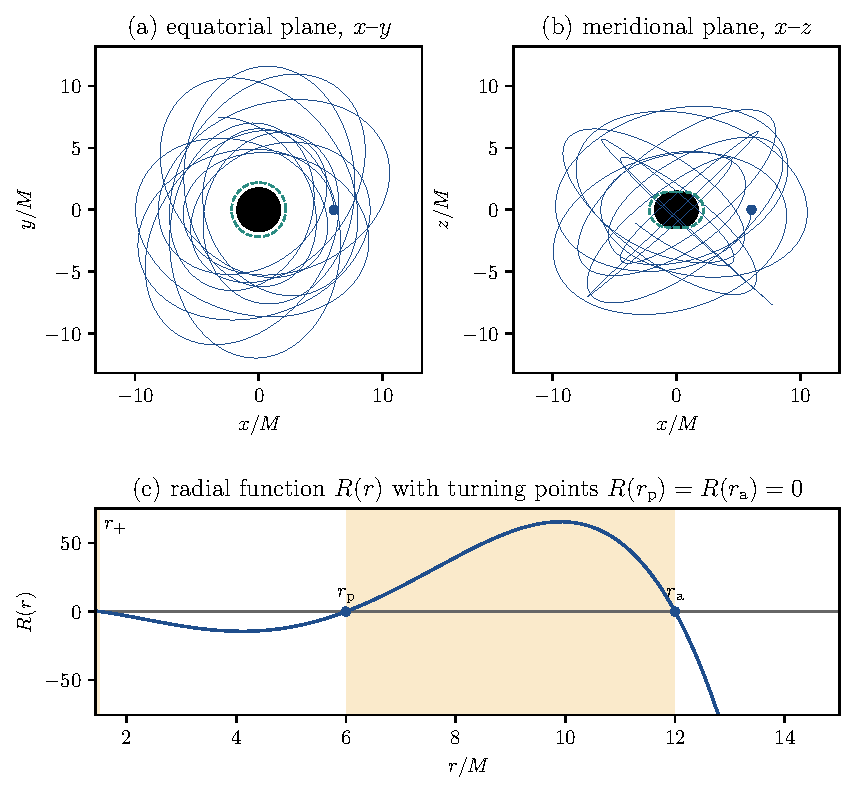
\includegraphics[width=0.95\textwidth]{kerr_orbit.pdf}
    \caption{A bound geodesic around a Kerr black hole with $a = 0.9M$, $r_{\mathrm{p}} = 6M$, $r_{\mathrm{a}} = 12M$ and $\iota = 45^\circ$, integrated up to $t = 2000M$. (a) Projection on the equatorial plane. (b) Projection on the meridional $x$--$z$ plane. (c) The radial function $R(r)$; the motion is allowed where $R \geq 0$ (shaded).}
    \label{Geo}
\end{figure}

Figure~\ref{Geo} shows the orbit with $a = 0.9$, $r_{\mathrm{p}} = 6$, $r_{\mathrm{a}} = 12$ and $\iota = 45^\circ$, for which $E = 0.948450$, $L = 2.309438$ and $Q = 5.333504$, followed up to coordinate time $t = 2000$ (proper time $\tau \approx 1640$). Positions are drawn at $x = \sqrt{r^2+a^2}\sin\theta\cos\phi$, $y = \sqrt{r^2+a^2}\sin\theta\sin\phi$ and $z = r\cos\theta$. The black region is the horizon $r = r_+$, the dashed curve is the outer boundary of the ergosphere, and the dot marks the starting point. Panel~(c) shows why the motion is confined: $R(r) \geq 0$ only between the turning points $r_{\mathrm{p}}$ and $r_{\mathrm{a}}$, and similarly $\Theta(\theta) \geq 0$ only for $45.1^\circ \leq \theta \leq 134.9^\circ$. The orbit does not close. Its periapsis advances within the orbital plane, as in the Schwarzschild case, and in addition the orbital plane itself precesses about the spin axis because of frame dragging (the Lense--Thirring effect). As a result, the projection on the equatorial plane gradually fills an annulus, and the meridional projection fills a band of latitudes.

An interactive version of this computation accompanies the report as the web page \texttt{kerr\_\allowbreak geodesics.html}. It uses the same equations \eqref{eq:mino-second}, with the fifth-order Dormand--Prince pair at relative tolerance $10^{-10}$. The reader can change $a$, the turning points and the inclination, or the constants $E$, $L$, $Q$ directly, and the orbit is animated in real time. It also covers plunging orbits and light rays ($\kappa = 0$).


\section{Extension to Charged Particle Dynamics}
So far we have studied neutral test particles, whose motion is integrable thanks to the four constants $\kappa$, $E$, $L$ and $Q$. Astrophysical black holes, however, are expected to be surrounded by magnetic fields, for example a large-scale field anchored in the accretion disk. Following Takahashi and Koyama~\cite{takahashi}, we now consider a test particle of charge $q$ in a stationary, axisymmetric, vacuum dipole magnetic field with four-potential $A_{\mu}(r,\theta)$, on a fixed Kerr background (the field is assumed too weak to change the geometry). In the Hamiltonian language of Section 3, the only change is that the kinetic momentum is replaced by $\pi_{\mu} - qA_{\mu}$, where $\pi_{\mu}$ is the canonical momentum:
\begin{equation}
    H = \frac{1}{2}g^{\mu\nu}(\pi_{\mu} - qA_{\mu})(\pi_{\nu} - qA_{\nu})
\end{equation}
Since $A_{\mu}$ does not depend on $t$ or $\phi$, both coordinates are still cyclic, so $E = -\pi_t$ and $L = \pi_{\phi}$ are still conserved; they now include contributions from $A_t$ and $A_{\phi}$. The Hamiltonian itself is also conserved, which again fixes the normalization $\kappa$. Once these three constants are fixed, what remains is a system with two degrees of freedom describing the poloidal motion in $(r,\theta)$. For a neutral particle, the Carter constant $Q$ is exactly the extra integral that makes this reduced system integrable, and it came from the separation of the Hamilton--Jacobi equation in $r$ and $\theta$. For a dipole field, $A_{\mu}$ couples $r$ and $\theta$, the separation fails, and in general no fourth constant of motion exists~\cite{takahashi}. Hence the poloidal motion is no longer integrable, and chaotic orbits can appear. The resulting orbits combine three kinds of motion: fast gyration around a magnetic field line, bouncing back and forth along the field line, and a slow drift in the toroidal ($\phi$) direction~\cite{takahashi}.

\begin{figure}[H]
    \centering
    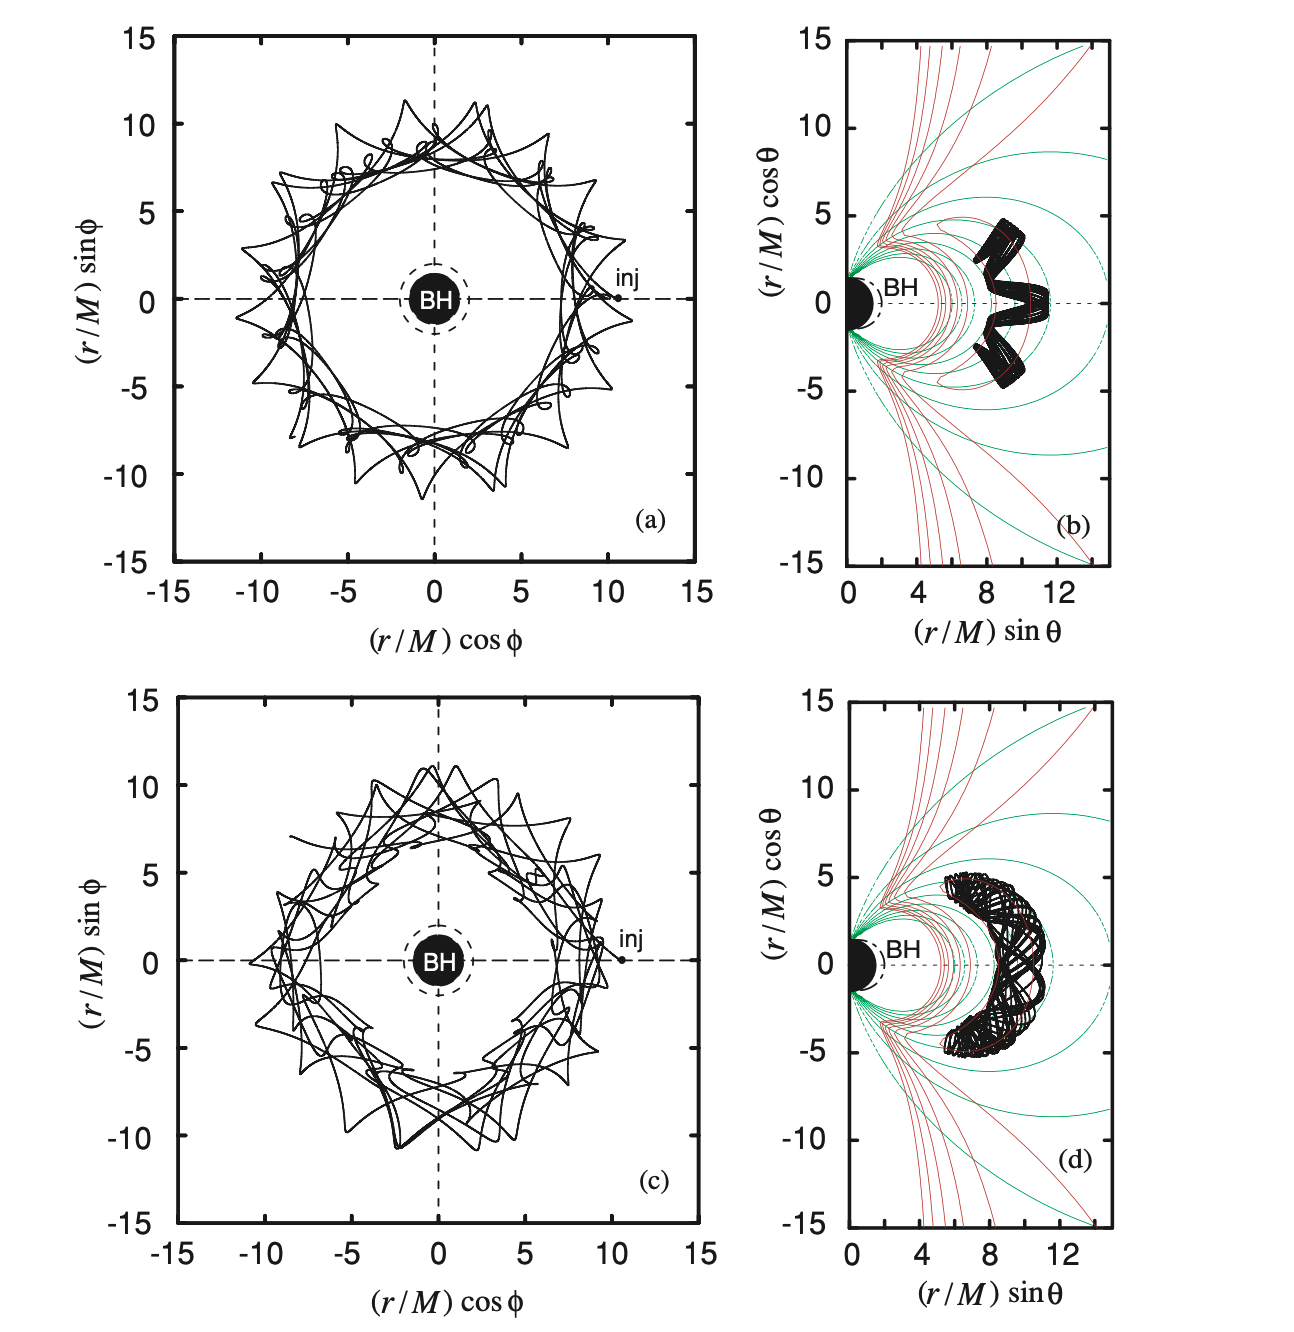
\includegraphics[width=0.8\textwidth]{geodesic2.png}
    \caption{Trajectories of a test charge around a Kerr black hole with $a=0.9M$. Left: projections onto the equatorial plane; right: projections onto the poloidal plane. Reproduced from Fig.~6 of~\cite{takahashi}.}
    \label{Geo2}
\end{figure}

Figure~\ref{Geo2} shows two such trajectories computed by Takahashi and Koyama~\cite{takahashi}. In the equatorial projections (left), the small loops and cusps are the gyration, while the overall circulation around the hole is the toroidal drift. The two rows have the same energy and angular momentum and differ only in the initial injection angle, yet their poloidal projections (right) look very different: in (b) the orbit stays on a thin, well-organized band, while in (d) it spreads over a much wider region. To decide whether an orbit is regular or chaotic, Takahashi and Koyama use Poincar\'e sections, and they find that frame dragging tends to regularize the motion: for rapidly rotating black holes some initial conditions give regular trajectories, while chaos dominates for slowly rotating ones~\cite{takahashi}. Such chaotic orbits could have implications for high-energy emission, particle acceleration, and the overall dynamics of magnetized plasma in black-hole environments.



\begin{thebibliography}{9}

\bibitem{oneill}
B.~O'Neill, 
\emph{The Geometry of Kerr Black Holes},
A K Peters/CRC Press, 1995.

\bibitem{schutz}
B.~Schutz,
\emph{A First Course in General Relativity},
2nd ed., Cambridge University Press, 2009.

\bibitem{wald}
R.~M.~Wald,
\emph{General Relativity},
The University of Chicago Press, 1984.

\bibitem{visser}
M.~Visser,
\emph{The Kerr Spacetime: A Brief Introduction},
arXiv:0706.0622 [gr-qc], 2007.

\bibitem{carter}
B.~Carter,
\emph{Global Structure of the Kerr Family of Gravitational Fields},
Phys. Rev. \textbf{174}, 1559 (1968).

\bibitem{goldstein}
H.~Goldstein,
\emph{Classical Mechanics}, 3rd ed.,
Addison Wesley, 2001, Chapter 10

\bibitem{mino}
Y.~Mino,
\emph{Perturbative approach to an orbital evolution around a supermassive black hole},
Phys. Rev. D \textbf{67}, 084027 (2003).

\bibitem{hairer}
E.~Hairer, S.~P.~N{\o}rsett and G.~Wanner,
\emph{Solving Ordinary Differential Equations I: Nonstiff Problems},
2nd ed., Springer, 1993.


\bibitem{takahashi}
M.~Takahashi and H.~Koyama,
\emph{Chaotic motion of Charged Particles in an Electromagnetic Field Surrounding a Rotating Black Hole},
arXiv:0807.0277v1 [astro-ph], 2008.

\end{thebibliography}












\end{document}
